\section{Calibración del campo y proyección a coordenadas métricas}
\label{sec:calibracion-campo-proyeccion-metricas}

En la \hyperref[sec:homografia-tecnologias]{Sección~\ref*{sec:homografia-tecnologias}} se introdujo el concepto de homografía y se describió PnLCalib como método para estimar la calibración geométrica del campo en vídeo broadcast. En esta sección se resume cómo se ha integrado dicha calibración dentro del sistema y, especialmente, qué estrategias de robustez han sido necesarias para poder usar la homografía como una señal fiable dentro del pipeline.

\subsection{Modelo utilizado y salida geométrica}

En este proyecto se utiliza PnLCalib en modo inferencia, con sus pesos pre-entrenados publicados por los autores en el repositorio oficial del proyecto \citep{PnLCalibRepo2024}, para estimar en cada frame la geometría del campo visible. A partir de las predicciones de puntos y líneas del terreno se obtiene una homografía $H_t$ que permite proyectar coordenadas en píxeles $(u,v)$ a coordenadas 2D sobre el plano del campo $(x,y)$, expresadas en unidades métricas.

La \hyperref[fig:calibracion-proyeccion-campo]{Figura~\ref*{fig:calibracion-proyeccion-campo}} ilustra este proceso. En la imagen original se muestran los puntos de referencia detectados sobre el terreno de juego, mientras que la vista cenital resultante permite visualizar la proyección de la escena sobre el plano del campo.

\begin{figure}[H]
\centering

\begin{minipage}{0.9\textwidth}
    \centering
    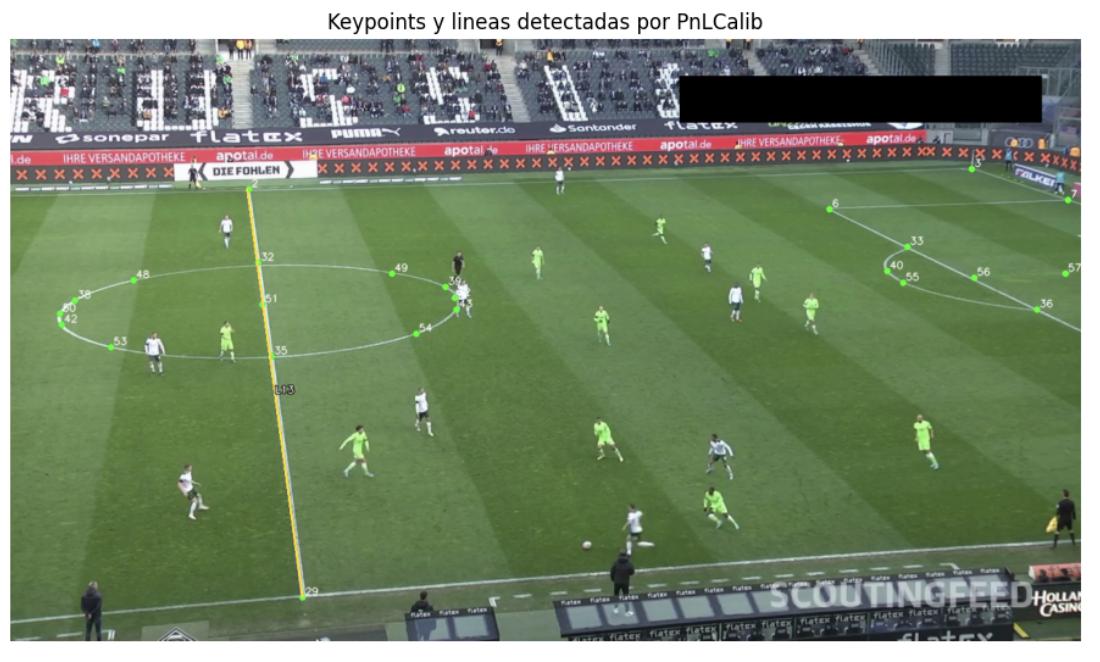
\includegraphics[width=\textwidth]{Imagenes/Propias/Puntos_referencia.png}
    \small \textbf{(a)} Puntos de referencia detectados sobre la imagen broadcast.
\end{minipage}

\vspace{0.4cm}

\begin{minipage}{0.9\textwidth}
    \centering
    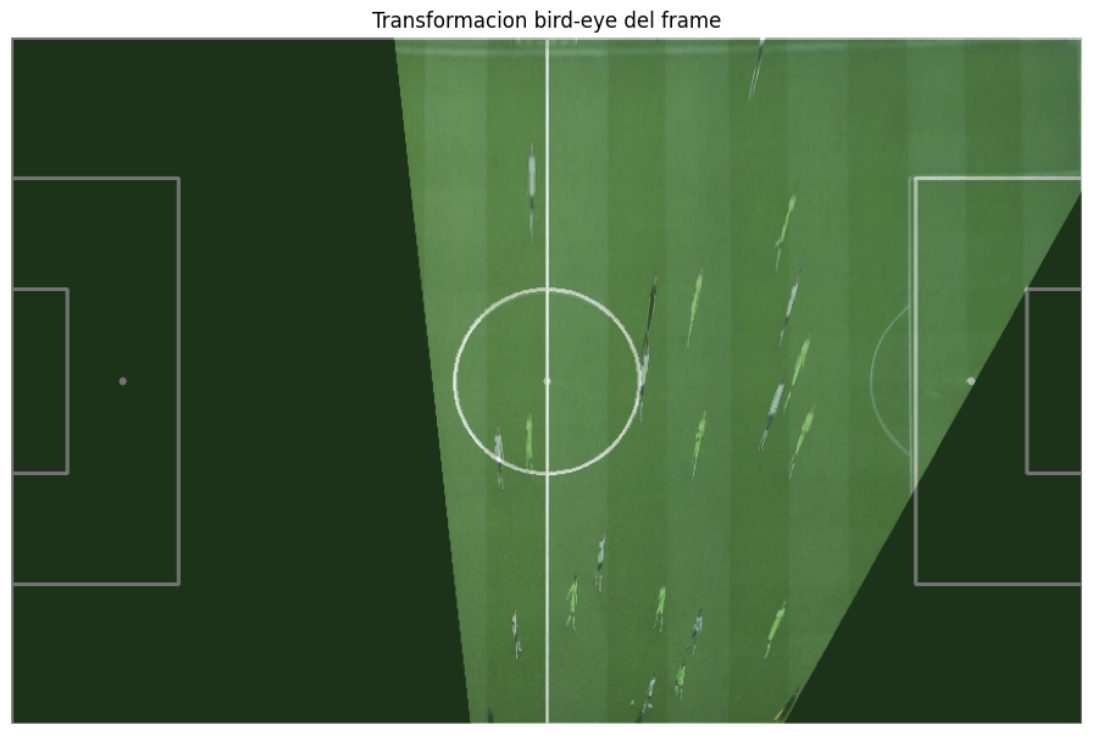
\includegraphics[width=\textwidth]{Imagenes/Propias/Bird_eye.png}
    \small \textbf{(b)} Proyección resultante en vista cenital del terreno de juego.
\end{minipage}

\caption[Calibración geométrica y proyección al plano del campo]{
Ejemplo de calibración geométrica del campo mediante PnLCalib. En (a) se muestran las referencias detectadas sobre la imagen broadcast y, en (b), la proyección de la escena sobre una representación 2D del terreno de juego.
}
\label{fig:calibracion-proyeccion-campo}
\end{figure}

Para proyectar la posición de un jugador no se utiliza el centro de su \textit{bounding box}, sino un punto que aproxima el contacto con el césped. En concreto, se emplea el punto central inferior de la caja, ligeramente desplazado hacia arriba:
\[
x = \frac{x_1 + x_2}{2}
\qquad
y = y_2 - 0.04 \cdot (y_2 - y_1)
\]
donde $(x_1,y_1,x_2,y_2)$ son las coordenadas de la \textit{bounding box}. Este punto se transforma mediante la homografía para obtener una posición $(x,y)$ en el campo.

La configuración de esta fase se resume en la \hyperref[tab:hiperparametros-referencia]{Tabla~\ref*{tab:hiperparametros-referencia}}, donde se recogen los parámetros utilizados por el módulo de proyección y sobre los que se irá hablando a lo largo de la sección.

\begin{table}[htbp]
\centering
\scriptsize
\setlength{\tabcolsep}{3pt}
\renewcommand{\arraystretch}{1.10}
\begin{tabularx}{\textwidth}{
>{\raggedright\arraybackslash}p{2.5cm}
>{\raggedright\arraybackslash}p{3.3cm}
>{\raggedright\arraybackslash}p{1.4cm}
>{\raggedright\arraybackslash}X
}
\toprule
\textbf{Bloque} & \textbf{Parámetro} & \textbf{Valor} & \textbf{Uso en pipeline} \\
\midrule

Redimensionado y punto de apoyo &
\texttt{bottom\_offset\_ratio} &
\texttt{0.04} &
Fija el desplazamiento vertical del punto proyectado sobre el césped. \\

\midrule

Umbrales base de inferencia &
\texttt{kp\_threshold} &
\texttt{0.30} &
Controla qué puntos de referencia se aceptan inicialmente. \\

&
\texttt{line\_threshold} &
\texttt{0.60} &
Controla qué líneas del campo se aceptan inicialmente. \\

&
\texttt{pnl\_refine} &
\texttt{false} &
Desactiva el refinamiento PnL adicional en esta configuración. \\

\midrule

Suavizado temporal &
\texttt{temporal\_blend} &
\texttt{0.20} &
Mezcla la homografía del frame actual con la anterior si la solución suavizada mantiene la calidad requerida. \\

\midrule

Búsqueda adaptativa &
\texttt{adaptive\_thresholds} &
\texttt{true} &
Activa varios intentos de calibración relajando umbrales. \\

&
\texttt{adaptive\_max\_attempts} &
\texttt{4} &
Número máximo de intentos por frame. \\

&
\texttt{adaptive\_kp\_step} &
\texttt{0.02} &
Reducción progresiva del umbral de puntos. \\

&
\texttt{adaptive\_line\_step} &
\texttt{0.05} &
Reducción progresiva del umbral de líneas. \\

&
\texttt{min. kp/line thresholds} &
\texttt{0.28/0.55} &
Límites inferiores hasta los que se relajan los umbrales. \\

\midrule

Soporte mínimo &
\texttt{min\_visible\_kp} &
\texttt{7} &
Número mínimo de puntos visibles requerido para aceptar una calibración. \\

&
\texttt{min\_visible\_lines} &
\texttt{1} &
Número mínimo de líneas visibles requerido para aceptar una calibración. \\

\midrule

Validación global &
\texttt{val\_score\_th} &
\texttt{0.56} &
Umbral mínimo del score compuesto de validación. \\

&
\texttt{val\_geometry\_fit\_min} &
\texttt{0.38} &
Mínimo requerido para la calidad del ajuste geométrico. \\

&
\texttt{val\_support\_quality\_min} &
\texttt{0.31} &
Mínimo requerido para la calidad del soporte geométrico. \\

&
\texttt{val\_coverage\_quality\_min} &
\texttt{0.18} &
Mínimo requerido para la cobertura de referencias. \\

\midrule

Validación geométrica &
\texttt{val\_reproj\_err\_px} &
\texttt{8.0} &
Rechaza soluciones con error de reproyección elevado. \\

&
\texttt{val\_H\_cond\_th} &
\texttt{1e8} &
Descarta homografías mal condicionadas. \\

&
\texttt{val\_kp\_world\_err\_m} &
\texttt{3.0} &
Limita el error métrico permitido en puntos. \\

&
\texttt{val\_line\_world\_err\_m} &
\texttt{4.0} &
Limita el error métrico permitido en líneas. \\

\midrule

Objetivos de cobertura &
\texttt{val\_target\_visible\_kp} &
\texttt{9} &
Objetivo de puntos visibles para considerar una calibración estable. \\

&
\texttt{val\_target\_visible\_lines} &
\texttt{4} &
Objetivo de líneas visibles. \\

&
\texttt{val\_target\_hull\_area} &
\texttt{0.18} &
Mide la cobertura espacial de los puntos en la imagen. \\

&
\texttt{val\_target\_x\_span} &
\texttt{0.55} &
Mide la extensión horizontal de las referencias. \\

&
\texttt{val\_target\_y\_span} &
\texttt{0.40} &
Mide la extensión vertical de las referencias. \\

&
\texttt{val\_target\_field\_cov} &
\texttt{0.20} &
Mide si las referencias cubren suficiente campo para estimar una homografía estable. \\

\bottomrule
\end{tabularx}

\caption[Hiperparámetros de calibración y proyección métrica]{
Hiperparámetros principales de la fase de calibración geométrica y proyección a coordenadas métricas.}
\label{tab:hiperparametros-referencia}
\end{table}

El valor final de estos hiperparámetros recogidos en la tabla se decidió mediante depuración iterativa y pruebas visuales sobre el vídeo de referencia. Este proceso de depuración se describe en la \hyperref[sec:evaluacion-heuristica-depuracion]{Sección~\ref*{sec:evaluacion-heuristica-depuracion}}.

\subsection{Problema de estabilidad: \textit{jitter} y sensibilidad a umbrales}

Durante las primeras pruebas se observó que la homografía estimada frame a frame era una señal poco estable: pequeñas variaciones en los puntos/líneas detectados producían cambios apreciables en la proyección, generando \textit{jitter} (vibración) tanto en la reconstrucción del campo como en las trayectorias proyectadas de los jugadores.

Este comportamiento ocurría principalmente con planos cerrados (esquinas o área), cuando la cámara realiza paneos o zooms rápidos, etc. 

Además, el método depende de umbrales de confianza para decidir qué puntos y líneas se consideran observados. En la práctica, fijar estos umbrales de forma única para todos los vídeos resulta difícil: con umbrales altos se obtienen menos referencias y muchos frames quedan sin homografía, mientras que con umbrales bajos se aceptan referencias ruidosas que degradan la calibración. Por tanto, la elección de umbrales tiene un componente arbitrario y el ``mejor'' valor depende del vídeo (calidad, resolución, iluminación y tipo de plano).

\subsection{Selección robusta de homografía: umbrales adaptativos y validación}

Para mejorar la robustez, se implementó una búsqueda por intentos con umbrales adaptativos sobre puntos clave y líneas. En cada frame se parte de una configuración base y se generan varios intentos relajando progresivamente los umbrales (hasta mínimos definidos), con el objetivo de aumentar el soporte geométrico en escenas difíciles.

El sistema evalúa todos los intentos y selecciona el mejor según un criterio lexicográfico: (i) aceptación de calidad, (ii) \textit{quality score} global y, en caso de empate, (iii) submétricas de ajuste geométrico, soporte y cobertura. Si ningún intento resulta aceptable, el frame se marca como no proyectable.

Esta estrategia permite adaptarse a distintos tipos de plano dentro del mismo partido (por ejemplo, plano general frente a plano cercano), y reduce la necesidad de calibrar manualmente umbrales por vídeo.

\subsubsection{Métricas de calidad y criterio de aceptación}

La homografía estimada no se utiliza de forma incondicional: se valida su calidad antes de habilitar su uso en tracking. El criterio que define la calidad de una homografía viene dado por la combinación de tres señales en un \textit{score} compuesto:
\begin{itemize}
    \item \textbf{Ajuste geométrico (\textit{geometry fit}):} incluye error de reproyección y chequeos de consistencia geométrica.
    \item \textbf{Soporte de referencias (\textit{support quality}):} cantidad y fiabilidad de puntos/líneas detectados.
    \item \textbf{Cobertura (\textit{coverage quality}):} distribución espacial/semántica de referencias para evitar soluciones concentradas o débiles.
\end{itemize}

Además del \textit{score} global, se aplican umbrales mínimos por submétrica y checks numéricos. Solo si el intento supera estos criterios se marca como aceptable para uso en tracking.

\subsubsection{Definición matemática de las métricas de calidad}

Sea un intento de calibración en un frame dado. Definimos funciones de normalización:
\[
clip(x)=\min(1,\max(0,x)),
\qquad
s_{\text{inv}}(e;\tau)=\frac{\tau}{\tau+e}
\]
\[
s_{\text{range}}(v;v_{\min},v_{\text{obj}})=
\mathrm{clip}\!\left(\frac{v-v_{\min}}{v_{\text{obj}}-v_{\min}}\right)
\]

Aquí, \({clip}\) acota cualquier valor al intervalo \([0,1]\), 
\(s_{\text{inv}}\) transforma un error \(e\) en una puntuación donde un valor mayor indica mejor calidad, y \(\tau\) controla la sensibilidad de esa transformación (en particular, \(s_{\text{inv}}=0.5\) cuando \(e=\tau\)), y \(s_{\text{range}}\) normaliza una magnitud \(v\) entre un mínimo y un objetivo, saturando el resultado en \([0,1]\).


Todas las submétricas se llevan a \([0,1]\), donde \(1\) es mejor.

\paragraph{1) Ajuste geométrico}
\[
G = 0.35\,s_{\text{rep}} + 0.15\,s_{\text{cond}} + 0.30\,s_{\text{kp-align}} + 0.20\,s_{\text{line-align}}
\]
con:
\[
s_{\text{rep}} = s_{\text{inv}}(e_{\text{rep}};\tau_{\text{rep}}),
\qquad
s_{\text{cond}}=
\mathrm{clip}\!\left(
1-\frac{\log_{10}(\kappa(H))}{\log_{10}(\kappa_{\max})}
\right),
\]
\[
s_{\text{kp-align}} = s_{\text{inv}}(e_{\text{kp-world}};\tau_{\text{kp-world}}),
\qquad
s_{\text{line-align}} = s_{\text{inv}}(e_{\text{line-world}};\tau_{\text{line-world}}).
\]

Donde \(e_{\text{rep}}\) es el error de reproyección devuelto por PnLCalib, \(\kappa(H)\) es el número de condición de la homografía \(H\), y \(e_{\text{kp-world}}\), \(e_{\text{line-world}}\) son errores medianos en metros tras proyectar puntos y líneas al campo. Los umbrales \(\tau_{\text{rep}}\), \(\kappa_{\max}\), \(\tau_{\text{kp-world}}\) y \(\tau_{\text{line-world}}\) corresponden a los valores de la Tabla~\ref{tab:hiperparametros-referencia} (respectivamente: \textit{val\_reproj\_err\_px}, \textit{val\_H\_cond\_th}, \textit{val\_kp\_world\_err\_m}, \textit{val\_line\_world\_err\_m}).

\(s_{\text{rep}}\) mide la consistencia global de la proyección en imagen (qué bien se reinyectan las referencias detectadas), \(s_{\text{cond}}\) mide la estabilidad numérica de la homografía estimada penalizando matrices mal condicionadas, \(s_{\text{kp-align}}\) mide la coherencia métrica de los puntos clave proyectados sobre el campo, y \(s_{\text{line-align}}\) mide la coherencia métrica de las líneas proyectadas en el plano del campo. En conjunto, estas submétricas capturan tanto el ajuste visual en imagen como la validez geométrica y la estabilidad numérica de la solución en coordenadas de juego.


\paragraph{2) Calidad del soporte de las referencias}
\[
S =
0.25\,s_{\text{kp-count}}
+ 0.20\,s_{\text{line-count}}
+ 0.15\,s_{\text{kp-conf}}
+ 0.10\,s_{\text{line-conf}}
+ 0.15\,s_{\text{kp-family}}
+ 0.15\,s_{\text{line-family}}.
\]

con:
\[
s_{\text{kp-count}}=
s_{\text{range}}(N_{kp};N_{kp}^{\min},N_{kp}^{obj}),\qquad
s_{\text{line-count}}=
s_{\text{range}}(N_{line};N_{line}^{\min},N_{line}^{obj}),
\]
\[
s_{\text{kp-conf}}=\frac{1}{N_{kp}}\sum_{i=1}^{N_{kp}} c^{kp}_i,\qquad
s_{\text{line-conf}}=\frac{1}{N_{line}}\sum_{j=1}^{N_{line}} c^{line}_j,
\]
\[
s_{\text{kp-family}}
=
\frac{1}{2}\left(\frac{B_x}{3}+\frac{B_y}{3}\right),
\]
\[
s_{\text{line-family}}
=
\mathrm{clip}\!\left(\frac{F_{\text{line}}}{3}\right).
\]

Donde \(N_{kp}\) y \(N_{line}\) son el número de \textit{keypoints} y líneas visibles; \(c^{kp}_i\) y \(c^{line}_j\) son sus confianzas individuales (devueltas por PnLCalib); \(B_x\) y \(B_y\) son el número de bandas ocupadas por los \textit{keypoints} en los ejes longitudinal y transversal del campo, tras dividir cada eje en tres intervalos; y \(F_{\text{line}}\) es el número de familias geométricas de líneas observadas, distinguiendo entre horizontales, verticales y estructura de portería.

Los umbrales y objetivos \(N_{kp}^{\min}\), \(N_{line}^{\min}\), \(N_{kp}^{obj}\) y \(N_{line}^{obj}\) corresponden a los valores de la Tabla~\ref{tab:hiperparametros-referencia} (respectivamente: \textit{min\_visible\_kp}, \textit{min\_visible\_lines}, \textit{val\_target\_visible\_kp}, \textit{val\_target\_visible\_lines}).

En esta puntuación, \(s_{\text{kp-count}}\) y \(s_{\text{line-count}}\) miden suficiencia de evidencia, \(s_{\text{kp-conf}}\) y \(s_{\text{line-conf}}\) miden fiabilidad media de las detecciones, \(s_{\text{kp-family}}\) mide si los \textit{keypoints} cubren zonas distintas del campo, y \(s_{\text{line-family}}\) mide si las líneas observadas pertenecen a familias geométricas variadas. En conjunto, estas submétricas intentan captar si la calibración se apoya en referencias no solo numerosas y fiables, sino también diversas.

\paragraph{3) Calidad de la cobertura del campo}
\[
C = 0.40\,s_{\text{img-hull}} + 0.20\,s_{\text{field-hull}} + 0.20\,s_{x\text{-span}} + 0.20\,s_{y\text{-span}}
\]
con:
\[
s_{\text{img-hull}}=\mathrm{clip}\!\left(\frac{A_{\text{img-hull}}}{A_{\text{img-hull}}^{\text{obj}}}\right),\qquad
s_{\text{field-hull}}=\mathrm{clip}\!\left(\frac{A_{\text{field-hull}}}{A_{\text{field-hull}}^{\text{obj}}}\right),
\]
\[
s_{x\text{-span}}=\mathrm{clip}\!\left(\frac{p_{x\text{-span}}}{p_{x\text{-span}}^{\text{obj}}}\right),\qquad
s_{y\text{-span}}=\mathrm{clip}\!\left(\frac{p_{y\text{-span}}}{p_{y\text{-span}}^{\text{obj}}}\right).
\]

Donde \(A_{\text{img-hull}}\) es la fracción de área del casco convexo de las referencias en imagen respecto al área total del frame; \(A_{\text{field-hull}}\) es la fracción de área del casco convexo de las referencias proyectadas en el campo respecto al área total del terreno de juego; y \(p_{x\text{-span}}\), \(p_{y\text{-span}}\) son las fracciones del ancho y del alto de la imagen cubiertas por la separación entre la referencia más extrema a izquierda/derecha y la más extrema arriba/abajo, respectivamente.

Los objetivos \(A_{\text{img-hull}}^{\text{obj}}\), \(A_{\text{field-hull}}^{\text{obj}}\), \(p_{x\text{-span}}^{\text{obj}}\) y \(p_{y\text{-span}}^{\text{obj}}\) corresponden a los valores de la Tabla~\ref{tab:hiperparametros-referencia} (respectivamente: \textit{val\_target\_hull\_area}, \textit{val\_target\_field\_cov}, \textit{val\_target\_} \textit{x\_span}, \textit{val\_target\_y\_span}).

En esta puntuación, \(s_{\text{img-hull}}\) mide cuánta superficie útil del frame queda anclada por referencias, \(s_{\text{field-hull}}\) mide su cobertura geométrica tras proyectarlas al plano del campo, y \(s_{x\text{-span}}\), \(s_{y\text{-span}}\) miden cuánto se extienden dichas referencias a lo ancho y a lo alto de la imagen. En conjunto, estas submétricas evalúan si la calibración está soportada por una cobertura amplia y bien distribuida.

\paragraph{Score final y criterio de aceptación:}

Si existe una homografía candidata válida, se calcula una puntuación global como combinación ponderada de las tres métricas anteriores:
\[
Q = 0.45\,G + 0.30\,S + 0.25\,C.
\]

Los umbrales de aceptación sobre estas métricas vienen dados por:
\[
G \ge G_{\min},\quad S \ge S_{\min},\quad C \ge C_{\min},\quad Q \ge Q_{\min},
\]
donde \(G_{\min}\), \(S_{\min}\), \(C_{\min}\) y \(Q_{\min}\) corresponden a los valores de la Tabla~\ref{tab:hiperparametros-referencia} (respectivamente: \textit{val\_geometry\_fit\_min}, \textit{val\_support\_quality\_min}, \textit{val\_coverage\_quality\_min}, \textit{val\_score\_th}).

Sin embargo, la aceptación final no depende solo de estas puntuaciones agregadas. Además, se aplican comprobaciones duras de validez: debe existir una homografía estimada, esta debe ser numéricamente válida y estar suficientemente bien condicionada, y el frame debe alcanzar al menos los mínimos de referencias visibles \(N_{kp}^{\min}\) y \(N_{line}^{\min}\). Por tanto, una solución puede obtener valores altos de \(G\), \(S\), \(C\) y \(Q\), pero aun así ser rechazada si falla alguna de estas condiciones duras.

\subsection{Suavizado temporal}

Incluso con homografías aceptables, puede existir variación frame a frame. Para reducir vibraciones se aplica un suavizado temporal opcional:
\[
H_t^{blend}=\alpha H_{t-1} + (1-\alpha)H_t^{raw}, \quad \alpha=0.20
\]

En la implementación, el resultado suavizado se conserva únicamente si también supera la validación de calidad y no reduce el \textit{quality score} frente a la solución no suavizada.

\subsection{Fallo controlado: \textit{fallback} cuando no hay homografía}

Por último, cuando no se consigue una homografía fiable, el pipeline no se detiene: se descarta la proyección métrica en ese frame y las fases posteriores continúan trabajando en coordenadas de imagen. Esta decisión evita que una calibración errónea contamine el resto del sistema.

En la \hyperref[fig:homography_frame]{Figura~\ref*{fig:homography_frame}} se muestra un ejemplo visual de la salida de esta fase para un frame del vídeo de prueba. En el panel de la izquierda aparecen las detecciones, los puntos y las líneas de referencia encontrados. En el de la derecha se muestra cómo quedan ubicadas las detecciones sobre el campo tras aplicar la homografía. El vídeo del resultado completo puede consultarse en \url{https://github.com/hectorgarciaa/narrador-futbol/output/homography/best/20260516_180637/homography.mp4}.
\begin{figure}[h]
    \centering
    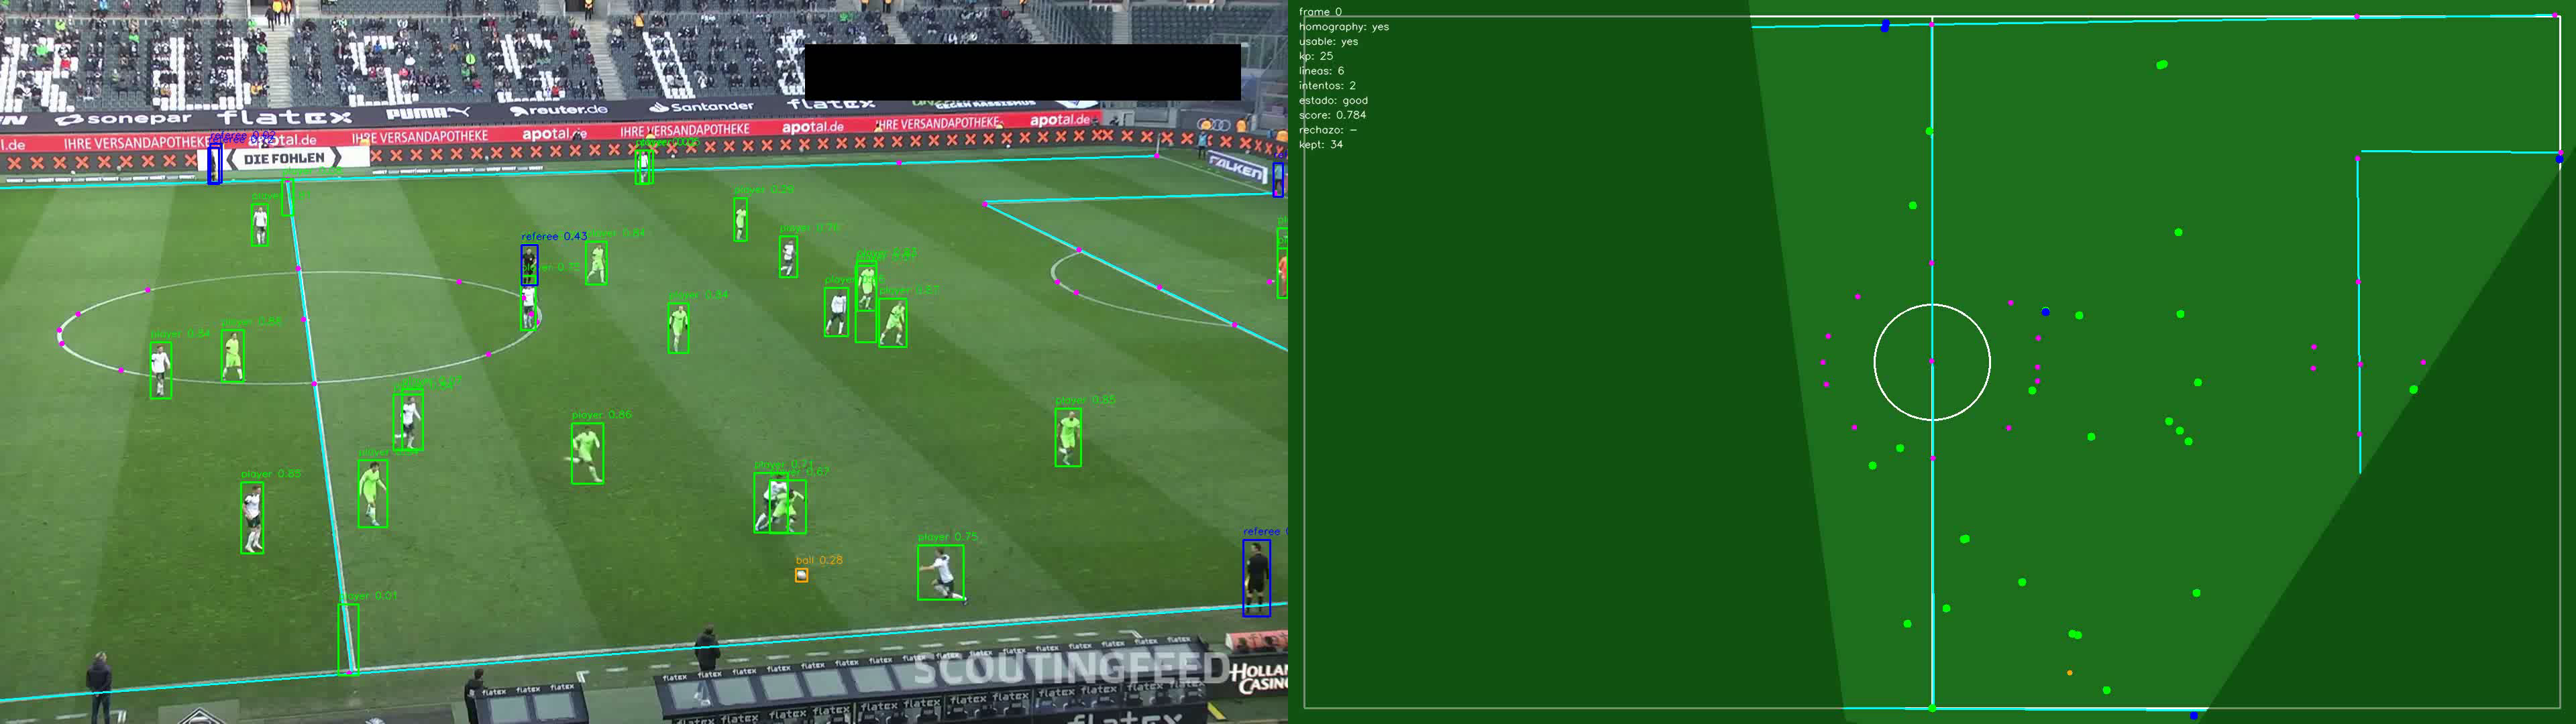
\includegraphics[width=0.85\textwidth]{Imagenes/Propias/homography_frame.png}
    \caption{Resultado visual de la fase de calibración del campo y proyección.}
    \label{fig:homography_frame}
\end{figure}
